\chapter{Concept design}
This chapter defines the global restraints on the concepts and presents an overview of the different concepts.

\section{Global restraints}
This section describes the global restraints on the concepts, as stated in the system requirements. 
\subsection{Myocardium}
\label{sec:myocardium}
To ensure compatibility to the clinical software, \textit{4DM}, the myocardium's cross-sectional shapes must be physiological; i.e. the \ac{HLA} and \ac{VLA} have the shape of a horseshoe and the \ac{SA} has the shape of a circle. 4DM requires these shapes to determine the contours and consequently determine the myocardial flow.
\subsection{Modality}
\label{sec:modality}
The main research question is based around the, relatively new in the Netherlands, D-SPECT's dynamic scanning. Therefore, the modality is bounded to the D-SPECT. As mentioned in section \ref{sec:concept_oper}, the D-SPECT is a suitable choice for myocardial perfusion imaging but still requires validation, which is the goal of the PhD research of which this project is part of.
\subsection{Tracer}
\label{sec:tracer}
The tracer and injection method are fixed due to clinical, 4DM, and dynamic scanning requirements. The clinical (and D-SPECT) protocol use \textsuperscript{99m}Tc (Technetium) Tetrofosmin for myocardial perfusion imaging. To ensure proper dynamic scanning results, the tracer must be injected with a pump. The pump can repeatedly inject tracer with identical volumes and injection speeds.
\subsection{Flow Type}
\label{sec:flowType}
Based on background information on the 4DM software, a decision has been made to use a non-pulsatile flow. The D-SPECT uses gated measurements such that images are extracted at the same point in time of the cardiac cycle. Furthermore, initial experiments with the D-SPECT, with non-pulsatile flow, have been performed on February 5, 2019. The prototype set-up from the individual project, with a dialysis tube, was placed in the D-SPECT and the TAC was extracted. This curve showed proper similarity to TACs extracted from patients.
\section{Concept overview}
Each concept is based on the mind map shown in appendix \ref{app:mind_map}. The following sections describe each aspect of the five main categories, respectively:
\begin{itemize}[noitemsep]
	\item Myocardium,
	\item Modality,
	\item Design,
	\item Tracer, and
	\item Flow.
\end{itemize}
\subsection{Myocardium}
The myocardium has two subcategories, the shape and the model. As described in section 
\subsection*{Shape}
As described in section \ref{sec:myocardium}, the shape of the myocardium is especially important for the 4DM software since it looks for the contours of the left ventricle's walls. Therefore, the shape of the myocardium is fixed (as per system requirements):

\begin{center}
\begin{minipage}{0.3\textwidth}
\begin{itemize}
	\item \ac{VLA}: Horseshoe (figure.
	\item \ac{HLA}: Horseshoe.
	\item \ac{SA}: circle.
\end{itemize}
\end{minipage}%
\begin{minipage}{0.3\textwidth}
\begin{figure}[H]
	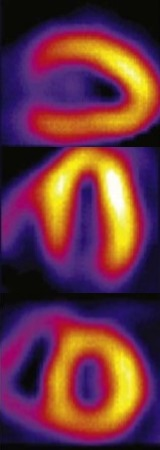
\includegraphics[height=5cm]{./images/stacked_shapes.jpg}
	\caption{Left ventricle's myocardial shapes: VLA, HLA, SA, respectively \citep{niwaz2015pres}}
	\label{fig:ventr_shape}
\end{figure}
\end{minipage}
\end{center}
\subsection*{Model}
\rrot{this section, depending on 4dm}.
The 4DM software offers different segment models in addition to the full 17-segment model, i.e. ...... The goal is to develop a phantom with 17 segments, fully compatible with 4DM. However, 4DM's ability to downscale to a fewer-segment model, provides the opportunity for a more simplified first prototype.
\subsection{Modality}
As described in section \ref{sec:modality}, the modality is fixed to the D-SPECT's dynamic scanning.
\subsection{Design}
The phantom can be designed in three different ways: using a 1-, 2-, or 4-chamber design. The 1-chamber design simulates only the left ventricle with the myocardium. The 2-chamber design simulates either the left and right ventricles, or the left atrium and ventricle. The other combinations, i.e. left ventricle and right atrium, and any combination without the left ventricle, does not hold any additional benefits. The 4-chamber design contains all heart chambers to simulate the flow as physiological as possible. A 3-chamber design is not considered since it has no physiological structure nor does it have an added benefit over a 1- or 2-chamber design.
\subsection{Tracer}
As described in section \ref{sec:tracer}, the tracer protocol is fixed.
\subsection{Flow}
\subsection*{Generator}
The flow in the phantom can be realised by a various of methods (or combinations thereof):
\begin{itemize} [noitemsep]
	\item Peristaltic pump,
	\item Gear pump,
	\item Air pressure,
	\item Dedicated myocardial generator,
	\item Branching aorta.
\end{itemize}
\subsection*{Supply}
The supply can be realised by a direct connection to the tap (water mains) or via a reservoir which can be filled directly from the tap or manually, e.g. using watering pots. In case of a closed circuit, see section \ref{sec:config}, the reservoir can be filled by the outflow of the phantom.
\subsection*{Disposal}
Proper disposal of contaminated, with nuclear tracer, will be a vital. Any fluid, or materials, that come into contact with the radioactive tracer, needs to be isolated for a period of multiple days. Spills should be avoided at all costs. Waste fluid can be stored in reservoirs, wheeled (closed) containers, or wheelie bins (Dutch "Kliko"). In case of a closed circuit, see section \ref{sec:config}, the outgoing flow can be directed to the input reservoir.

\subsection*{Configuration}
\label{sec:config}
The flow set-up can be designed in either a closed circuit or open circuit. The closed circuit characterises itself by having no disposal flow, see figure \ref{fig:closed_circ}. The optional filter can extract, if possible, the tracer from the perfusate such that first pass perfusion is realised. Otherwise, the tracer is recirculated which causes the bolus to disappear. An alternative is an open circuit, see figure \ref{fig:open_circ}, which guarantees first pass perfusion due to the absence of any form of recirculation.
\begin{minipage}{0.5\textwidth}
\begin{figure}[H]
	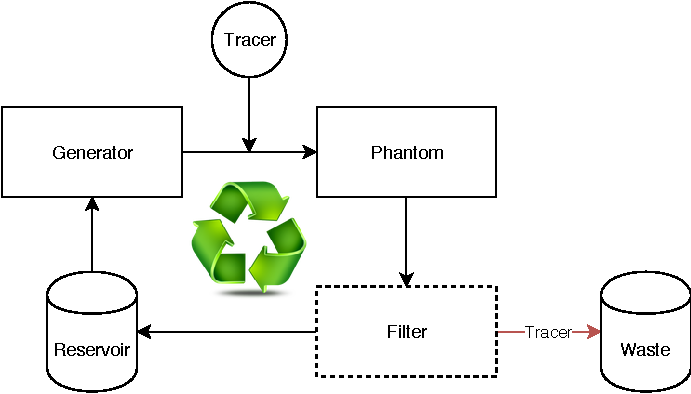
\includegraphics[width=\linewidth]{./images/concept_design_closedCircuit.pdf}
	\caption{Closed circuit schematic design}
	\label{fig:closed_circ}
\end{figure}
\end{minipage}%
\begin{minipage}{0.5\textwidth}
\begin{figure}[H]
	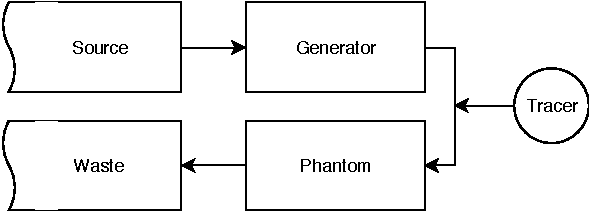
\includegraphics[width=\linewidth]{./images/concept_design_openCircuit.pdf}
	\caption{Open circuit schematic design}
	\label{fig:open_circ}
\end{figure}
\end{minipage}
\subsection*{Type}
As described in section \ref{sec:flowType}, the flow type is fixed.
\subsection*{Perfusate}
Two types of perfusate can be chosen from: water and blood-mimicking fluid (BMF). Water is most practical since it is available in a steady supply. However, BMF is more physiological since it is of the same viscosity as human blood but needs to be made before performing any experiments. In an open circuit configuration, see section \ref{sec:config}, BMF will be rapidly put into the waste collection making it very costly. In an closed circuit, if the tracer can be filtered from the BMF, it will potentially be a more accurate simulation.
\section{Concepts}
\subsection{Concept 1}
\subsection{Concept 2}
\subsection{Summary}
\begin{table}[H]
\caption{Concept overview}
\begin{tabular}{l|llll}
\textbf{}                                                  &                               & \multicolumn{1}{c}{Concept 1} & Concept 2                & Concept x                                     \\ \hline
\multicolumn{1}{c|}{}                                      & \cellcolor{red}Shape &\cellcolor{red}      & \cellcolor{red} & \multicolumn{1}{l|}{\cellcolor{red}} \\
\multicolumn{1}{c|}{\multirow{-2}{*}{\textbf{Myocardium}}} & Model                         &                               &                          & \multicolumn{1}{l|}{}                         \\
\textbf{Modality}                                          & \cellcolor{red}      & \cellcolor{red}      & \cellcolor{red} & \multicolumn{1}{l|}{\cellcolor{red}} \\
\textbf{Design}                                            &                               &                               &                          & \multicolumn{1}{l|}{}                         \\
\textbf{Tracer}                                            & \cellcolor{red}      & \cellcolor{red}      & \cellcolor{red} & \multicolumn{1}{l|}{\cellcolor{red}} \\
                                                           & Generator                     &                               &                          & \multicolumn{1}{l|}{}                         \\
                                                           & Supply                        &                               &                          & \multicolumn{1}{l|}{}                         \\
                                                           & Disposal                      &                               &                          & \multicolumn{1}{l|}{}                         \\
                                                           & Configuration                 &                               &                          & \multicolumn{1}{l|}{}                         \\
                                                           & \cellcolor{red}Type  & \cellcolor{red}      & \cellcolor{red} & \multicolumn{1}{l|}{\cellcolor{red}} \\
\multirow{-6}{*}{\textbf{Flow}}                            & Perfusate                     &                               &                          & \multicolumn{1}{l|}{}                         \\ \cline{2-5} 
\end{tabular}
\end{table}
